\newpage
\section{1 семестр}
	\subsection*{1}
	Показать, что $\mathbb{Z}^2$ изоморфно $\mathbb{Z}^{2 \: \star}$\\
	Где $\mathbb{Z}^{2 \: \star} \ = \ \mathbb{Z}^2 / (0, 0)$
	
	\subsection*{2}
	Докажите, что: $|\Delta(F)| = |\Delta(f)|$\\
	Где:\\
	$
	\Delta \: \text{--- дискриминант}\\
	f(x,y) = ax^2 + bxy + cy^2\\
	F(x,y) = f(\alpha x + \beta y,\: \gamma x + \delta y)
	$
	
	\subsection*{3}
	А)\\
	Доказать через цепные дроби
	\begin{gather*}
	|\omega - \frac{p_n}{q_n} | < \frac{1}{q^2_n}
	\end{gather*}
	где $\omega$ -- трансцендентное число\\
	\\
	Б)\\
	\begin{gather*}
	|\omega - \frac{p_n}{q_n} | < \frac{1}{q^k_n} \quad \forall k \in \mathbb{N} 
	\end{gather*}
	Подробнее о таких приближениях можно прочесть в книгах:\\
	"Теория диофантовых приближений"\ Дж.В.С.Касселс\\
	"Теория диофантовых приближений"\ С.Ленг.
	
	\subsection*{4}
	Площадь фундаментального параллелограмма не зависит от базиса\\
	$S(e_1,\ e_2) = S(e_1,\ e_2 + e_1 \cdot \lambda )$
	\\
	Фундаментальный параллелограмм -- параллелограмм, чьи вершины лежат в узлах решётки, других узлов внутри и на границе нет
	
	\subsection*{5}
	$(e,p)$ -- базис решетки, $f$ - самый короткий вектор из $L$\\
	Доказать, что проекция $\text{pr}_{e^{\perp}} L$ -- это решетка на прямой $e^{\bot}$\\
	Т.е. $\exists p: \ \mathbb{Z}_[p] = \text{pr}_{e^{\perp}} L$\\
	Где: \\
	$\text{pr}_{e^{\perp}} L$ --  решетка на прямой $e^{\perp}$
	
	\subsection*{6}
	$(e,f)$ -- базис решетки\\
	Базис Коркина-Золотарева\\
	$p^r_{e^{\bot}} f = p$\\
	$f = p + \mu e \quad \mu \in \mathbb{R}$\\
	можно ли выбрать $f$ так, что $|\mu| \leq \frac{1}{2}$
	
	\subsection*{7}
	$f(x,y) = (x - \lambda y)(x - \lambda^{\backslash} y)$\\
	$\lambda, \lambda^{\backslash}$ -- есть корни
	$L_1 = x - \lambda y, \ L_2 = x - \lambda^{\backslash} y$
		
	\subsection*{8}
	Если одно из $\lambda$ рационально, то $\exists p,q: \ f(p,q) = 0 \quad (p,q) \in (\mathbb{R}^2)^{\star}$
	
	\subsection*{9}
	\begin{figure}[h]
		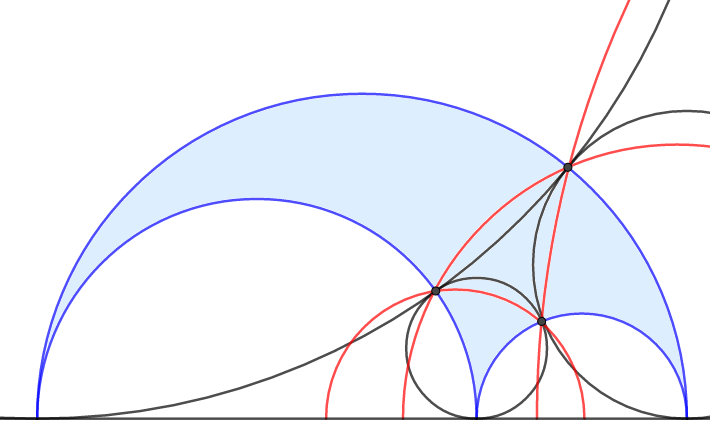
\includegraphics[width=0.75\linewidth]{pic1}
	\end{figure}
	Почему таким образом(как на картинке) можно построить любой неделимый вектор\\
	Пояснение условия: почему в группе Коксетера присутствуют все неделимые вектора, которые можно получить из заданных базис-векторов $e_1, e_2$
	
	\subsection*{10}
	Почему в группе Коксетера граница между участками плоскости(странами) - дерево, степень каждой вершины которой равна $3$
	\newpage
	\subsection*{11}
	Река в группе Коксетера --- линия разделяющая положительные и отрицательные значения форм $f(x,y)$ на данных $(e_1, e_2)$. Поясните в каких случаях река единственна и какие значения принимает $f(x,y)$ в клетках граничащих с рекой.	
	\\
	\begin{figure}[h]
		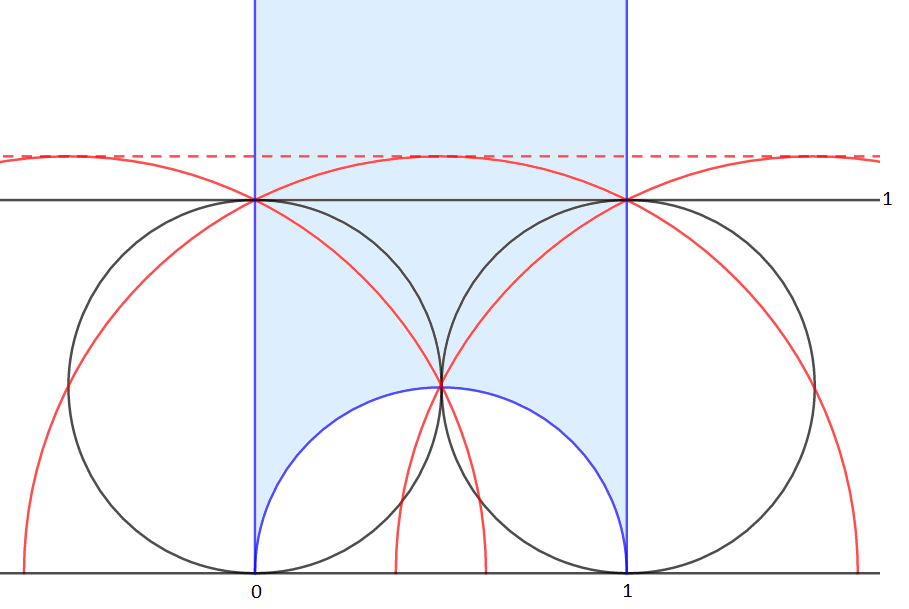
\includegraphics[width=0.75\linewidth]{pic2}
	\end{figure}
	Пример реки для формы $f(x,y) = x^2 - 3y^2$

	\subsection*{12}
	Любой неделимой вектор решетки можно дополнить до базиса
		
	
\begin{comment}
	\newpage
	\section{2 модуль}
	
	\newpage
	\section{3 модуль}
	
	\newpage
	\section{4 модуль}
\end{comment}	
